
\documentclass{article}
\usepackage{tikz}
\usetikzlibrary{positioning}
\newdimen\nodeDist
\nodeDist=55mm
\begin{document}

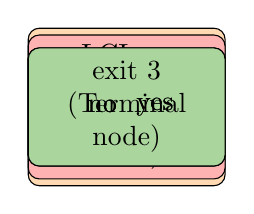
\begin{tikzpicture}[
    node/.style={%
      draw,
      rectangle,
    },
  ]

\tikzstyle{s1} = [rectangle, rounded corners, minimum width=2.5cm, minimum height=2cm,text width=2cm, text centered, draw=black, fill=orange!30]

\tikzstyle{s2} = [rectangle, rounded corners, minimum width=2.5cm, minimum height=1.5cm,text width=2cm, text centered, draw=black, fill=red!30]

\tikzstyle{s3} = [rectangle, rounded corners, minimum width=2.5cm, minimum height=1.5cm,text width=2cm, text centered, draw=black, fill={rgb:red,2;green,5;blue,1; white,10}]

    \node [s1,] (A) {IDS $>$ 13.5? (Root node)};
    \path (A) ++(-135:\nodeDist) node [s3] (B) {exit 1 (Terminal node)};
    \path (A) ++(-45:\nodeDist) node [s2] (C) {LCIanx $>$ 0.3604? (Decision node)};
    \path (C) ++(-135:\nodeDist) node [s3] (D) {exit 2 (Terminal node)};
    \path (C) ++(-45:\nodeDist) node [s3] (E) {exit 3 (Terminal node)};

    \draw (A) -- (B) node [left,pos=0.25] {no}(A);
    \draw (A) -- (C) node [right,pos=0.25] {yes}(A);
    \draw (C) -- (D) node [left,pos=0.25] {no}(A);
    \draw (C) -- (E) node [right,pos=0.25] {yes}(A);
\end{tikzpicture}

\end{document}


\begin{figure}[!htbp]
\centering
\def\layersep{2.5cm}
\usetikzlibrary{shapes.geometric, arrows}

\newdimen\nodeDist
\nodeDist=55mm

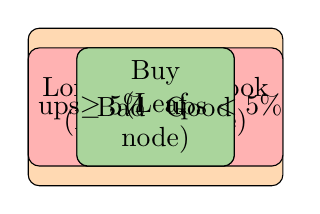
\begin{tikzpicture}[node distance=2cm]

\tikzstyle{s1} = [rectangle, rounded corners, minimum width=2.5cm, minimum height=2cm,text width=3cm, text centered, draw=black, fill=orange!30]

\tikzstyle{s2} = [rectangle, rounded corners, minimum width=3cm, minimum height=1.5cm,text width=3cm, text centered, draw=black, fill=red!30]

\tikzstyle{s3} = [rectangle, rounded corners, minimum width=2cm, minimum height=1.5cm,text width=1.5cm, text centered, draw=black, fill={rgb:red,2;green,5;blue,1; white,10}]

    \node [s1,] (A) {Stock price (Root node)};
    \path (A) ++(-135:\nodeDist) node [s3] (B) {Buy (Leaf node)};
    \path (A) ++(-45:\nodeDist) node [s2] (C) {Long-term outlook  (Internal node)};
    \path (C) ++(-135:\nodeDist) node [s3] (D) {Sell (Leaf node)};
    \path (C) ++(-45:\nodeDist) node [s3] (E) {Buy (Leaf node)};

    \draw (A) -- (B) node [left,pos=0.25] { ups$ \ge 5\%$}(A);
    \draw (A) -- (C) node [right,pos=0.25] {ups $<5\%$ }(A);
    \draw (C) -- (D) node [left,pos=0.25] {Bad}(A);
    \draw (C) -- (E) node [right,pos=0.25] {Good}(A);

\end{tikzpicture}
\caption{Example of a decision tree structure}
\label{fig:dtflow}
\end{figure}
